In the article, the symmetries of the IM-I is omitted as its fit is much worse than the other two candidate models. Although, the emphasis is on the comparison between the PLM and the IM-II the symmetries of the IM-I have also been calculated. A summary of all the calculated symmetries is presented below (Tab \ref{tab:sym_tab}).


\begin{table}[htbp!]
\begin{center}
\caption[Summary of the symmetries]{\textbf{Summary of the symmetries}. The models, their generators and the non-trivial symmetries are presented from left to right. }
\begin{tabular}{||c|c|c||}
\hline\hline
 & & \\
\textit{Model} & Generators & Non-trivial\\
& & Symmetries\\
& & \\
 \hline\hline
& & \\
PLM & $X_{1,0}=\left(\frac{t^{\gamma+1}}{\gamma}\right)\partial_t+Rt^{\gamma}\partial_R$& \\
  & $X_{1,1}=t\partial_t$& $\Gamma_{1,1}(\epsilon):(t,R)\mapsto \left(te^{\epsilon},R\right)$\\
  & $X_{1,2}=t^{\gamma}\partial_R$ & $\Gamma_{1,2}(\epsilon):(t,R)\mapsto (t,R+\epsilon t^{\gamma})$\\
 & & \\
 \hline
 & & \\
 IM-II & $X_2=e^{\alpha t}\exp\left(-e^{-\alpha(t-\tau)}\right)\partial_t$ & $\Gamma_2(\epsilon):(t,R)\mapsto\left(\tau-\dfrac{\ln\left(\ln\left(\left|\alpha e^{\alpha\tau}\epsilon-\exp\left(e^{-\alpha (t-\tau)}\right)\right|\right)\right)}{\alpha},R\right)$\\
 & & \\
 \hline
 & & \\
 IM-I & $X_{3,0}=\frac{1}{\alpha}e^{\alpha t}\partial_t+Re^{\alpha t}\partial_R$& \\
 & $X_{3,1}=\partial_t$& $\Gamma_{3,1}(\epsilon):(t,R)\mapsto(t+\epsilon,R)$\\
 & $X_{3,2}=e^{\alpha t}\partial R$& $\Gamma_{3,2}:(t,R)\mapsto (t,R+\epsilon e^{\alpha t}) $\\
 & & \\
 \hline\hline
 \end{tabular}
\label{tab:sym_tab}
\end{center}
\end{table}



A commonality between the three models is that all non-trivial generators are uni-directional. Both the PLM and the IM-I have $R$-directional symmetries, i.e. $\Gamma_{1,2}$ and $\Gamma_{3,2}$ whereas the IM-II
 merely has a $t$-directional symmetry in $\Gamma_{2}$. The action of the non-trivial symmetries of the PLM (Fig \ref{fig:PLM}), the IM-II (Fig \ref{fig:IM-II}) and the IM-I (Fig \ref{fig:IM-I}) respectively is illustrated below.

\begin{figure}[htbp!]
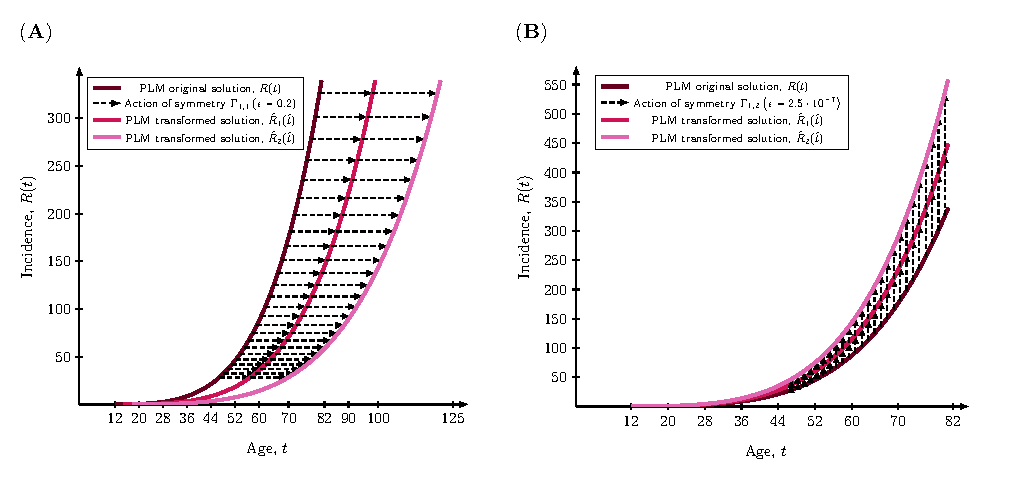
\includegraphics[width=\textwidth]{FigS2}
\caption[Action of the non-trivial symmetries of the PLM]{\textit{Action of the non-trivial symmetries of the PLM}. The original curve which is generated from the PLM with parameters $(A,\gamma)=(7.742,4.528)$ is transformed twice with the two non-trivial symmetries of the PLM. (\textbf{A}) The $t$-directional scaling symmetry $\Gamma_{1,1}$ with transformation parameter $\epsilon=0.2$. (\textbf{B}) The $R$-directional symmetry $\Gamma_{1,2}$ with transformation parameter $\epsilon=2.5\cdot 10^{-7}$.}
\label{fig:PLM}
\end{figure}

\begin{figure}[htbp!]
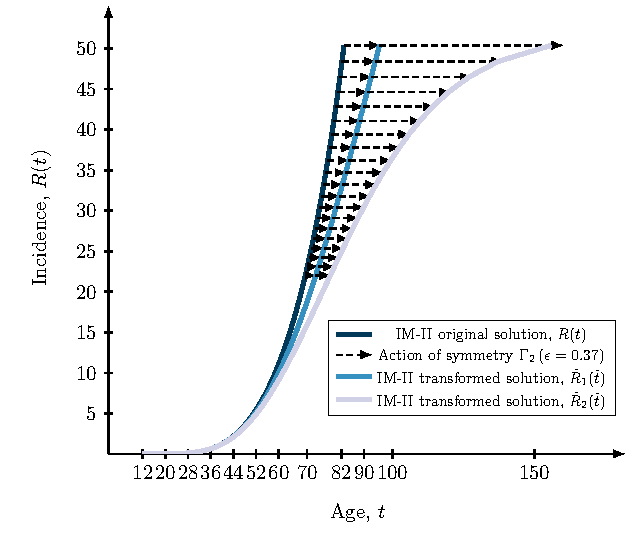
\includegraphics[width=\textwidth]{FigS3}
\caption[Action of the non-trivial symmetry of the IM-II]{\textit{Action of the non-trivial symmetry of the IM-II}. The original curve which is generated from the IM-II with parameters $(\ln(A),\tau,\alpha)=(3.4822,67.1564,0.044)$ is transformed twice with the non-trivial symmetry of the IM-II. More precisely, the original curve is transformed twice with the $t$-directional symmetry $\Gamma_{2}$ with transformation parameter $\epsilon=0.37$.}
\label{fig:IM-II}
\end{figure}




\begin{figure}[htbp!]
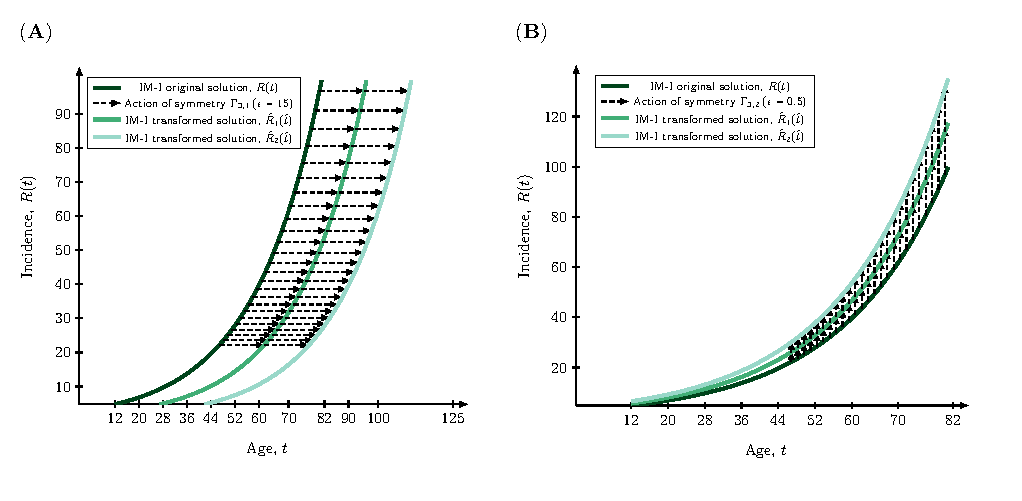
\includegraphics[width=\textwidth]{FigS1}
\caption[Action of the non-trivial symmetries of the IM-I]{\textit{Action of the non-trivial symmetries of the IM-I}. The original curve which is generated from the IM-I with parameters $(A,\alpha)=(2.090,0.044)$ is transformed twice with the two non-trivial symmetries of the PLM. (\textbf{A}) The $t$-directional translation symmetry $\Gamma_{3,1}$ with transformation parameter $\epsilon=15$. (\textbf{B}) The $R$-directional symmetry $\Gamma_{3,2}$ with transformation parameter $\epsilon=0.5$.}
\label{fig:IM-I}
\end{figure}